\documentclass{standalone}
\usepackage{tikz}
\usetikzlibrary{patterns, positioning}

\begin{document}
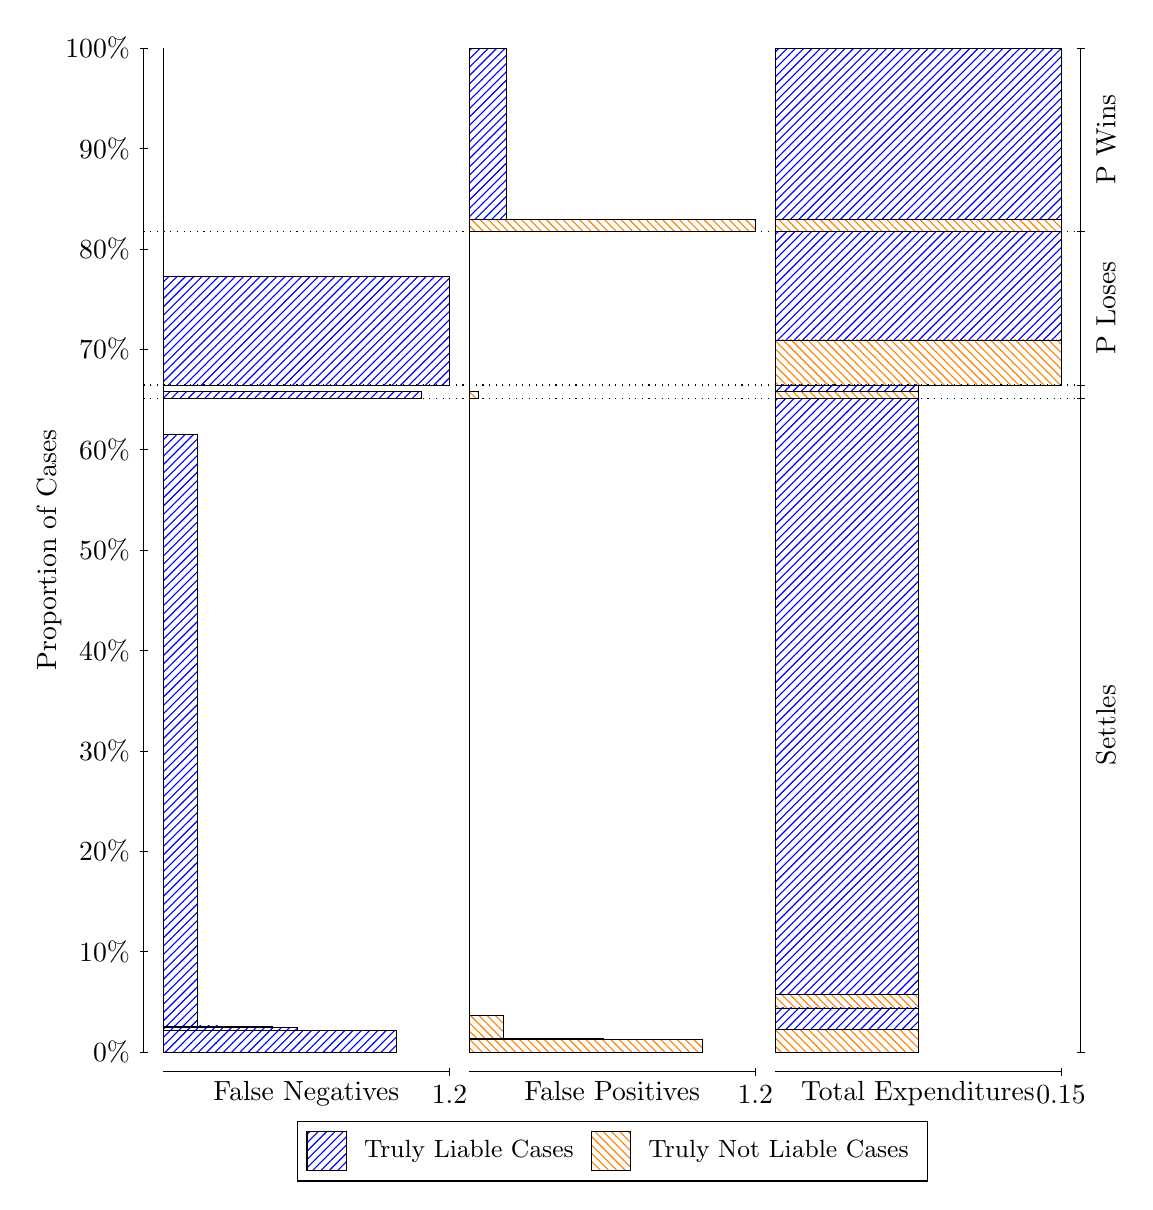
\begin{tikzpicture}
\draw[black, very thin] (1.5,1.75) -- (1.5,14.5);
\node[rotate=90, anchor=center] at (0.3, 8.125) {Proportion of Cases};
\draw[black, very thin] (1.45,1.75) -- (1.55,1.75);
\node[anchor=east] at (1.45, 1.75) {0\%};
\draw[black, very thin] (1.45,3.025) -- (1.55,3.025);
\node[anchor=east] at (1.45, 3.025) {10\%};
\draw[black, very thin] (1.45,4.3) -- (1.55,4.3);
\node[anchor=east] at (1.45, 4.3) {20\%};
\draw[black, very thin] (1.45,5.575) -- (1.55,5.575);
\node[anchor=east] at (1.45, 5.575) {30\%};
\draw[black, very thin] (1.45,6.85) -- (1.55,6.85);
\node[anchor=east] at (1.45, 6.85) {40\%};
\draw[black, very thin] (1.45,8.125) -- (1.55,8.125);
\node[anchor=east] at (1.45, 8.125) {50\%};
\draw[black, very thin] (1.45,9.4) -- (1.55,9.4);
\node[anchor=east] at (1.45, 9.4) {60\%};
\draw[black, very thin] (1.45,10.675) -- (1.55,10.675);
\node[anchor=east] at (1.45, 10.675) {70\%};
\draw[black, very thin] (1.45,11.95) -- (1.55,11.95);
\node[anchor=east] at (1.45, 11.95) {80\%};
\draw[black, very thin] (1.45,13.225) -- (1.55,13.225);
\node[anchor=east] at (1.45, 13.225) {90\%};
\draw[black, very thin] (1.45,14.5) -- (1.55,14.5);
\node[anchor=east] at (1.45, 14.5) {100\%};

\draw[black, very thin] (13.4,1.75) -- (13.4,14.5);
\draw[black, very thin] (13.35,1.75) -- (13.45,1.75);
\node[anchor=west] at (13.35, 1.75) {};
\draw[black, very thin] (13.35,10.054) -- (13.45,10.054);
\node[anchor=west] at (13.35, 10.054) {};
\draw[black, very thin] (13.35,10.221) -- (13.45,10.221);
\node[anchor=west] at (13.35, 10.221) {};
\draw[black, very thin] (13.35,12.173) -- (13.45,12.173);
\node[anchor=west] at (13.35, 12.173) {};
\draw[black, very thin] (13.35,14.5) -- (13.45,14.5);
\node[anchor=west] at (13.35, 14.5) {};

\draw[black, very thin, pattern color=blue, pattern=north east lines] (1.75,1.75) rectangle (4.712,2.0193);
\draw[black, very thin, pattern color=blue, pattern=north east lines] (1.75,2.0193) rectangle (3.4482,2.0671);
\draw[black, very thin, pattern color=blue, pattern=north east lines] (1.75,2.0671) rectangle (3.1322,2.0719);
\draw[black, very thin, pattern color=blue, pattern=north east lines] (1.75,2.0719) rectangle (2.8163,2.0767);
\draw[black, very thin, pattern color=blue, pattern=north east lines] (1.75,2.0767) rectangle (2.5004,2.0818);
\draw[black, very thin, pattern color=blue, pattern=north east lines] (1.75,2.0818) rectangle (2.1844,9.5898);
\draw[black, very thin, pattern color=orange, pattern=north west lines] (1.75,9.5898) rectangle (1.75,10.054);
\draw[black, very thin, pattern color=blue, pattern=north east lines] (1.75,10.054) rectangle (5.0279,10.135);
\draw[black, very thin, pattern color=orange, pattern=north west lines] (1.75,10.135) rectangle (1.75,10.221);
\draw[black, very thin, pattern color=blue, pattern=north east lines] (1.75,10.221) rectangle (5.3833,11.601);
\draw[black, very thin, pattern color=orange, pattern=north west lines] (1.75,11.601) rectangle (1.75,12.173);
\draw[black, very thin, pattern color=orange, pattern=north west lines] (1.75,12.173) rectangle (1.75,12.325);
\draw[black, very thin, pattern color=blue, pattern=north east lines] (1.75,12.325) rectangle (1.75,14.5);
\draw[black, very thin, pattern color=orange, pattern=north west lines] (5.6333,1.75) rectangle (8.5953,1.9115);
\draw[black, very thin, pattern color=orange, pattern=north west lines] (5.6333,1.9115) rectangle (8.2793,1.9125);
\draw[black, very thin, pattern color=orange, pattern=north west lines] (5.6333,1.9125) rectangle (7.9634,1.9136);
\draw[black, very thin, pattern color=orange, pattern=north west lines] (5.6333,1.9136) rectangle (7.6475,1.9146);
\draw[black, very thin, pattern color=orange, pattern=north west lines] (5.6333,1.9146) rectangle (7.3315,1.9249);
\draw[black, very thin, pattern color=orange, pattern=north west lines] (5.6333,1.9249) rectangle (6.0678,2.2143);
\draw[black, very thin, pattern color=blue, pattern=north east lines] (5.6333,2.2143) rectangle (5.6333,10.054);
\draw[black, very thin, pattern color=orange, pattern=north west lines] (5.6333,10.054) rectangle (5.7518,10.141);
\draw[black, very thin, pattern color=blue, pattern=north east lines] (5.6333,10.141) rectangle (5.6333,10.221);
\draw[black, very thin, pattern color=orange, pattern=north west lines] (5.6333,10.221) rectangle (5.6333,10.794);
\draw[black, very thin, pattern color=blue, pattern=north east lines] (5.6333,10.794) rectangle (5.6333,12.173);
\draw[black, very thin, pattern color=orange, pattern=north west lines] (5.6333,12.173) rectangle (9.2667,12.325);
\draw[black, very thin, pattern color=blue, pattern=north east lines] (5.6333,12.325) rectangle (6.1072,14.5);
\draw[black, very thin, pattern color=orange, pattern=north west lines] (9.5167,1.75) rectangle (11.333,2.0394);
\draw[black, very thin, pattern color=blue, pattern=north east lines] (9.5167,2.0394) rectangle (11.333,2.3087);
\draw[black, very thin, pattern color=orange, pattern=north west lines] (9.5167,2.3087) rectangle (11.333,2.4836);
\draw[black, very thin, pattern color=blue, pattern=north east lines] (9.5167,2.4836) rectangle (11.333,10.054);
\draw[black, very thin, pattern color=orange, pattern=north west lines] (9.5167,10.054) rectangle (11.333,10.141);
\draw[black, very thin, pattern color=blue, pattern=north east lines] (9.5167,10.141) rectangle (11.333,10.221);
\draw[black, very thin, pattern color=orange, pattern=north west lines] (9.5167,10.221) rectangle (13.15,10.794);
\draw[black, very thin, pattern color=blue, pattern=north east lines] (9.5167,10.794) rectangle (13.15,12.173);
\draw[black, very thin, pattern color=orange, pattern=north west lines] (9.5167,12.173) rectangle (13.15,12.325);
\draw[black, very thin, pattern color=blue, pattern=north east lines] (9.5167,12.325) rectangle (13.15,14.5);
\draw[black, dotted] (1.5,10.054) -- (13.4,10.054);
\draw[black, dotted] (1.5,10.221) -- (13.4,10.221);
\draw[black, dotted] (1.5,12.173) -- (13.4,12.173);
\draw[black, very thin] (1.75,1.5) -- (5.3833,1.5);
\node[anchor=north] at (3.5667, 1.5) {False Negatives};
\draw[black, very thin] (5.3833,1.45) -- (5.3833,1.55);
\node[anchor=north] at (5.3833, 1.45) {1.2};

\draw[black, very thin] (5.6333,1.5) -- (9.2667,1.5);
\node[anchor=north] at (7.45, 1.5) {False Positives};
\draw[black, very thin] (9.2667,1.45) -- (9.2667,1.55);
\node[anchor=north] at (9.2667, 1.45) {1.2};

\draw[black, very thin] (9.5167,1.5) -- (13.15,1.5);
\node[anchor=north] at (11.333, 1.5) {Total Expenditures};
\draw[black, very thin] (13.15,1.45) -- (13.15,1.55);
\node[anchor=north] at (13.15, 1.45) {0.15};

\node[black, centered, rotate=90] at (13.72, 5.9021) {Settles};

\node[black, centered, rotate=90] at (13.72, 11.197) {P Loses};
\node[black, centered, rotate=90] at (13.72, 13.337) {P Wins};

\draw (7.449999999999999,1.5) node[draw=none] (baseCoordinate) {};
\begin{scope}[align=center]
        \matrix[scale=0.5, draw=black, below=0.5cm of baseCoordinate, nodes={draw}, column sep=0.1cm]{
            \node[rectangle, draw, minimum width=0.5cm, minimum height=0.5cm, pattern=north east lines, pattern color=blue] {}; &
            \node[draw=none, font=\small] (B) {Truly Liable Cases}; &
            \node[rectangle, draw, minimum width=0.5cm, minimum height=0.5cm, pattern=north west lines, pattern color=orange] {}; &
            \node[draw=none, font=\small] (B) {Truly Not Liable Cases}; \\
            };
\end{scope}

\end{tikzpicture}
\end{document}